% ------------------------------------------------------------------------------
% TYPO3 CMS 7.4 - What's New - Chapter "Introduction" (French Version)
%
% @author	Michael Schams <schams.net>
% @license	Creative Commons BY-NC-SA 3.0
% @link		http://typo3.org/download/release-notes/whats-new/
% @language	French
% ------------------------------------------------------------------------------
% LTXE-CHAPTER-UID:		9dc37b9a-9fad14c3-bf7eabfd-82b83622
% LTXE-CHAPTER-NAME:	Introduction
% ------------------------------------------------------------------------------

\section{Introduction}
\begin{frame}[fragile]
	\frametitle{Introduction}

	\begin{center}\huge{Introduction}\end{center}
	\begin{center}\huge{\color{typo3darkgrey}\textbf{Faits}}\end{center}

\end{frame}

% ------------------------------------------------------------------------------
% LTXE-SLIDE-START
% LTXE-SLIDE-UID:		8765ab4f-72a439d6-78edb3d2-4f66b6b5
% LTXE-SLIDE-ORIGIN:	3cc566cf-d7166203-45a36415-7c8e8ebf English
% LTXE-SLIDE-ORIGIN:	5d8622ac-37911548-171bf8ec-5add4ed5 German
% LTXE-SLIDE-TITLE:		TYPO3 CMS 7.4 - The Facts
% ------------------------------------------------------------------------------
\begin{frame}[fragile]
	\frametitle{Introduction}
	\framesubtitle{TYPO3 CMS 7.4 - Faits}

	\begin{itemize}
		\item Date de sortie~: 4 Août 2015
		\item Type de sortie~: "Sprint Release"
		\item Slogan~: Embrace, Innovate, Deliver
		\item Axe principal~: Backend Overhaul Vol 2
	\end{itemize}

\end{frame}

% ------------------------------------------------------------------------------
% LTXE-SLIDE-START
% LTXE-SLIDE-UID:		7d078da5-fd92f1de-20c5c655-0fd3b8ef
% LTXE-SLIDE-ORIGIN:	6746e3bc-a8575d0c-e1681766-d0d78911 English
% LTXE-SLIDE-ORIGIN:	9da27f39-55d99c31-9ee9136a-20d96c0e German
% LTXE-SLIDE-TITLE:		System Requirements
% ------------------------------------------------------------------------------
\begin{frame}[fragile]
	\frametitle{Introduction}
	\framesubtitle{Prérequis système}

	\begin{itemize}
		\item PHP*~:\tabto{3cm}v5.5.0 - v5.6.x
		\item MySQL~:\tabto{3cm}v5.5.x - v5.6.x (pas de mode strict)
		\item Espace disque~:\tabto{3cm}min. 200 Mo
		\item Configuration PHP~:

			\begin{itemize}
				\item memory\_limit >= 128M
				\item max\_execution\_time >= 240s
				\item L'option de compilation \texttt{--disable-ipv6} \underline{NE} doit \underline{PAS} être utilisée
			\end{itemize}

		\item Le backend nécessite IE >= 9 ou tout autre navigateur moderne

	\end{itemize}

	\vspace{.8cm}
	*) Plus d'information~: \href{http://typo3.org/news/article/php-minimum-requirements-for-typo3-cms-7/}{Prérequis PHP minimum pour TYPO3 CMS 7 (en anglais)}

\end{frame}

% ------------------------------------------------------------------------------
% LTXE-SLIDE-START
% LTXE-SLIDE-UID:		7d68887a-d78057be-9c4ba67a-31a6966b
% LTXE-SLIDE-ORIGIN:	081f8b1d-b8f58841-dccf8d1d-148fd25d English
% LTXE-SLIDE-ORIGIN:	dbbfebbe-fb43ddb8-bca9ae69-716b8a0f German
% LTXE-SLIDE-TITLE:		Development And Release Timeline
% ------------------------------------------------------------------------------
\begin{frame}[fragile]
	\frametitle{Introduction}
	\framesubtitle{Chronologie des développements et sorties}

	\begin{figure}
		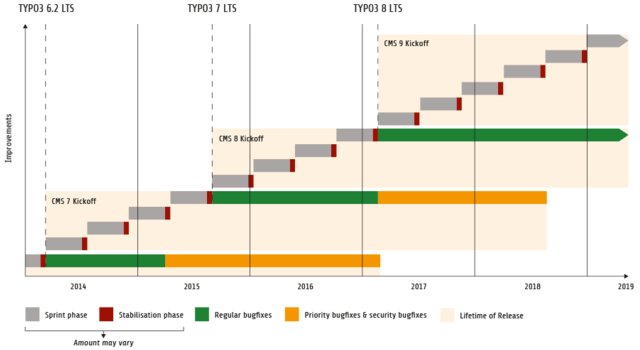
\includegraphics[width=0.90\linewidth]{Introduction/ReleaseAgenda.png}
	\end{figure}

\end{frame}

% ------------------------------------------------------------------------------
% LTXE-SLIDE-START
% LTXE-SLIDE-UID:		9a3faa63-b994ab0d-a6bf7d85-84a72a69
% LTXE-SLIDE-ORIGIN:	a5555bb0-f1f8031f-f271766a-2dbc1b08 English
% LTXE-SLIDE-ORIGIN:	e359142e-e7c10774-5d851da9-b26a275b German
% LTXE-SLIDE-TITLE:		TYPO3 CMS Roadmap
% ------------------------------------------------------------------------------
\begin{frame}[fragile]
	\frametitle{Introduction}
	\framesubtitle{Feuille de route TYPO3 CMS}

	Dates de sortie estimées et axes principaux~:

	\begin{itemize}
		\item v7.0 \tabto{1.0cm}02/Déc./2014\tabto{3.4cm}Backend Overhaul Vol 1
		\item v7.1 \tabto{1.0cm}24/Fév./2015\tabto{3.4cm}Core Cleanup \& Streamlining
		\item v7.2 \tabto{1.0cm}28/Avr./2015\tabto{3.4cm}Frontend
		\item v7.3 \tabto{1.0cm}16/Juin/2015\tabto{3.4cm}Package Ecosystem, Composer
		\item
			\begingroup
				\color{typo3orange}
					v7.4 \tabto{1.0cm}04/Août/2015\tabto{3.4cm}Backend Overhaul Vol 2
			\endgroup

		\item v7.5 \tabto{1.0cm}29/Sep./2015\tabto{3.4cm}\textit{(à déterminer…)}
		\item v7.6 \tabto{1.0cm}xx/xxx/2015\tabto{3.4cm}\textbf{TYPO3 CMS 7 LTS} (Long Term Release)
	\end{itemize}

	\smaller
		\url{https://typo3.org/typo3-cms/roadmap/}\newline
		\url{http://typo3.org/news/article/embrace-and-innovate-typo3-cms-7/}
	\normalsize

\end{frame}

% ------------------------------------------------------------------------------
% LTXE-SLIDE-START
% LTXE-SLIDE-UID:		256b9aa2-e5ae8c50-26f5da3e-06705bbb
% LTXE-SLIDE-ORIGIN:	5ef3ad6d-b72464d3-6a2867a6-298cb382 English
% LTXE-SLIDE-ORIGIN:	c8966352-3e5159b9-f0e3ea35-9d4455ef German
% LTXE-SLIDE-TITLE:		Installation
% ------------------------------------------------------------------------------
\begin{frame}[fragile]
	\frametitle{Introduction}
	\framesubtitle{Installation}

	\begin{itemize}
		\item Procédure officielle d'installation sous Linux/Mac OS X\newline
			(DocumentRoot considéré \texttt{/var/www/site/htdocs}):
		\begin{lstlisting}
			$ cd /var/www/site
			$ wget --content-disposition get.typo3.org/7.4
			$ tar xzf typo3_src-7.4.0.tar.gz
			$ cd htdocs
			$ ln -s ../typo3_src-7.4.0 typo3_src
			$ ln -s typo3_src/index.php
			$ ln -s typo3_src/typo3
			$ touch FIRST_INSTALL
		\end{lstlisting}

		\item Liens symboliques sous Microsoft Windows:

			\begin{itemize}
				\item Utiliser \texttt{junction} sous Windows XP/2000
				\item Utiliser \texttt{mklink} sous Windows Vista et Windows 7
			\end{itemize}

	\end{itemize}
\end{frame}

% ------------------------------------------------------------------------------
% LTXE-SLIDE-START
% LTXE-SLIDE-UID:		7f2cdafa-c21ee990-4c4f446b-2c95ccfc
% LTXE-SLIDE-ORIGIN:	12551741-9cb07199-fb3614d0-1a242a5f English
% LTXE-SLIDE-ORIGIN:	af099855-2b970b2b-89ed7d02-7219b2b9 German
% LTXE-SLIDE-TITLE:		Upgrade to TYPO3 CMS 7
% ------------------------------------------------------------------------------
\begin{frame}[fragile]
	\frametitle{Introduction}
	\framesubtitle{Mise à jour vers TYPO3 CMS 7.x}

	\begin{itemize}
		\item Les mises à jour sont possibles seulement depuis TYPO3 CMS 6.2 LTS
		\item TYPO3 CMS < 6.2 doivent être mis à jour vers la 6.2 LTS en premier
	\end{itemize}

	\begin{itemize}

		\item Instructions de mise à jour~:\newline
			\smaller\url{http://wiki.typo3.org/Upgrade#Upgrading_to_7.4}\normalsize
		\item Guide TYPO3 officiel «~TYPO3 Installation and Upgrading~»~:
			\smaller\url{http://docs.typo3.org/typo3cms/InstallationGuide}\normalsize
		\item De manière générale~:
			\begin{itemize}
				\item Vérifier les prérequis système \small(PHP, MySQL, etc)
				\item Examiner \textbf{deprecation\_*.log} de l'ancienne instance TYPO3
				\item Mettre à jour toutes les extensions vers leurs dernières versions
				\item Déployer les nouvelles sources et exécuter l'assistant de mise à jour de l'Install Tool
				\item Examiner le module de démarrage des utilisateurs backend (optionnel)
			\end{itemize}
	\end{itemize}

\end{frame}

% ------------------------------------------------------------------------------
